
%%%%%%%%%%%%%%%%%%%%%%%%%%%%%%%%%%%%%%%%%%%%%%%%%%%%%%%%%%%%%%%%%%%%%%%%%%%%%%%%
%%%%%%%%%%%%%%%%%%%%%%%%%%%%%%%%%%%%%%%%%%%%%%%%%%%%%%%%%%%%%%%%%%%%%%%%%%%%%%%%
% DESIGN AND IMPLEMENTATION %
%%%%%%%%%%%%%%%%%%%%%%%%%%%%%%%%%%%%%%%%%%%%%%%%%%%%%%%%%%%%%%%%%%%%%%%%%%%%%%%%

\cleardoublepage
\chapter{Design and implementation}
\label{chap:implementation}

In this chapter, all the phases of the project mentioned above are detailed. The evolution of each process and its description, as well as the problems encountered, are described in each section.

\section{Documentation and training}
\label{sec:documentation}

The beginning of the project was mainly based on a period of training and documentation. During the first months of this work, as we described in Chapter~\ref{chap:objectives}, it was necessary a previous formation in aspects such as CT, the Scratch language, Dr. Scratch and its architecture or the concept of bad smells, among others.

After this process, we decided to present an article about the Dr. Scratch tool in the 3rd Scientix Conference\footnote{http://www.scientix.eu/es/conference/scx3} celebrated in Brussels, Belgium. This paper, ``Dr. Scratch: Assess Scratch projects for Computational Thinking skills'', was composed of a single page and summarized the general definition of Dr. Scratch and its main characteristics. This congress entailed the first contact with this researching project. 

\section{General architecture of Dr. Scratch} 
\label{sec:arquitectura}

Dr. Scratch is a client-server tool which analyzes the JSON file of a Scratch project. Its main architecture can be shown in Figure~\ref{fig:architecture}. Clients make HTTP requests to the server, which was allocated in a virtual machine of the Azure platform with Ubuntu 14.04.2 LTS as operative system. It was possible thanks to a free subscription of Microsoft. However, this subscription was over when we were developing the new version and it had to be migrated to the Google Cloud Platform, which will be detailed in Section~\ref{subsec:mig_to_google}. 

 \begin{figure}
    \centering
    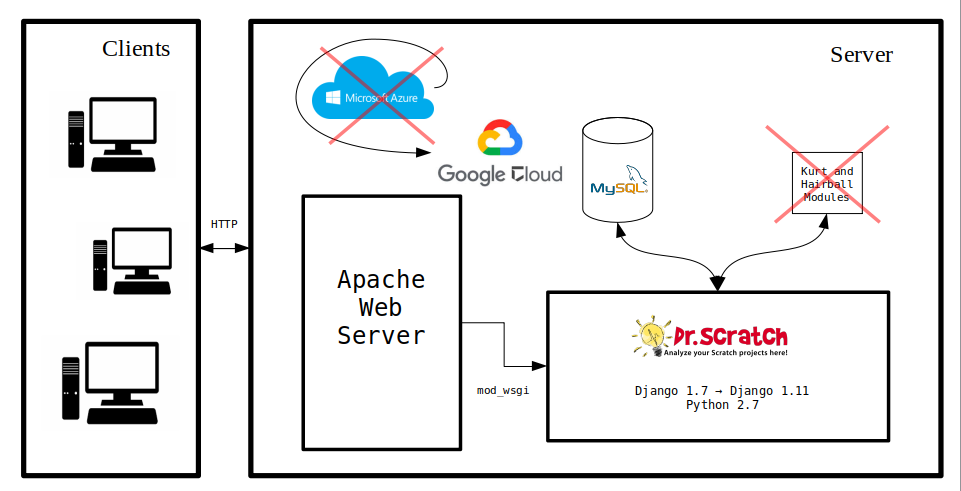
\includegraphics[width=12cm,                         keepaspectratio]{img/Client_Server.png}
    \caption{General architecture of Dr. Scratch.}
    \label{fig:architecture}
\end{figure}

The version 2.4.10 of Apache Web Server was installed inside of the virtual machine of Azure, the same as the \textit{mod\_wsgi} module, which connects Azure with Django.

On the other hand, in order to collect the information, Dr. Scratch used the version 5.5.43 of the MySQL database. 

Hairball and Kurt modules were also installed in the virtual machine because they were necessary for the analysis of the Scratch projects. Kurt is a Python library useful for working with the Scratch project files. Hairball analyzes the JSON file of the Scratch projects and returns the assessment of the CT development and the total number of bad smells that the project has. Hairball analyzes the blocks of the projects through different plugins.


\subsection{Dr. Scratch 3.0}
\label{subsec:newversion}

The starting point of this phase was the update of the Django version. The version 1.7 was obsolete, so we migrated the code to Django 1.11 LTS. This process was mainly based on minor modifications to the code and it could be done easily and quickly.

On the other hand, the Scratch community announced the launch of the new Scratch 3.0 version in the coming months. From this point, we investigated its main changes. 

The most important modification was the structure of the JSON file of the Scratch projects. Hairball and Kurt modules were not compatible with the new format. Therefore, the first step was to modify these modules, since they only supported Scratch 1.4 and Scratch 2.0 versions. 

In order to simplify the software of Dr. Scratch, we decided to remove the modules instead of updating them to the new version -because we thought that it was an easier and more efficient solution. In its place, we programmed some new scripts with the same functionality, but integrated into the main code. In other words, the objective of this process was to develop different scripts which analyzed the CT development and the total number of bad smells in the Scratch projects and integrate them into the Dr. Scratch code.

Once that the functionality of Hairball and Kurt was replicated, we integrated the scripts in the main code of Dr. Scratch and removed the modules. We describe in more detail each of the scripts below. 

\subsubsection{Mastery}
\label{subsubsec:mastery}

The \textit{analyzer.py} script analyzes the blocks of the JSON file and returns the punctuation of each of the seven categories of the CT which the Hairball module analyzed, the total mastery and the level of competence of the project. Each category -flow control, data representation, abstraction, user interactivity, synchronization, parallelism and logic- is scored from 0 to 3 points, depending on the type of blocks. The total punctuation is the sum of the points of each category. Therefore, the range of the total mastery is from 0 to 21 points. Depending on the final mastery, the script differentiates three types of profiles (the same as Hairball module): Basic (0 to 7 points), Developing (8 to 15 points) and Proficiency (16 to 21 points). In Table~\ref{table:competence_level} is detailed the evaluation of the competence levels for each CT concept~\cite{moreno2015dr}.

  \begin{table}
    \begin{center}
    \begin{tabular}{|c|p{3.5cm}|p{3.5cm}|p{3.5cm}|}
    \hline
     & \multicolumn{3}{|c|}{\textbf{Competence Level}} \\ \cline{2-4}
    \textbf{CT Concept} & \textbf{Basic} & \textbf{Developing} & \textbf{Proficiency} \\ 
    & (1 Point) & (2 Points) & (3 Points) \\ \hline  
    \textbf{Flow control} & Sequence of blocks. & Use of \textit{repeat} or \textit{forever} blocks. & Use of \textit{repeat until} block. \\ \hline
    \textbf{Data representation} & Modifiers of sprites properties (looks, motion). & Operations on variables. & Operations on lists. \\ \hline
    \textbf{Abstraction} & More than one script or more than one sprite. & Definition of blocks. & Use of clones. \\ \hline
    \textbf{User interactivity} & Use of \textit{green flag} block. & Use of \textit{key pressed}, \textit{sprite clicked}, \textit{ask and wait} or \textit{mouse} blocks. & Use of video or audio sensing blocks. \\ \hline
    \textbf{Synchronization} & Use of \textit{wait} block. & Use of \textit{broadcast} and \textit{receive messages}, \textit{stop all} or \textit{stop program} blocks. & Use of \textit{wait until}, \textit{when backdrop change to} or \textit{broadcast and wait} blocks. \\ \hline
    \textbf{Parallelism} & Two scripts on \textit{green flag}. & On the same sprite, two scripts on \textit{key pressed} or on \textit{sprite clicked}. & Two scripts start with the same multimedia event, \textit{when broadcast received}, \textit{when backdrop switches to} or \textit{create clone}. \\ \hline
    \textbf{Logic} & Use of \textit{if} block. & Use of \textit{if else} block. & Use of operator blocks. \\ \hline
  \end{tabular}
  \caption{Competence levels for each CT concept.}
  \label{table:competence_level}
 \end{center}
\end{table}

\subsubsection{Sprite naming}
\label{subsubsec:sprite_naming}

The \textit{spriteNaming.py} script analyzes the presence of names by default in the sprites (Sprite1, Sprite2, \ldots, SpriteN) in the JSON file of the Scratch projects. It returns the total number of default sprite names found in the program, as well as a list with all of them.

\subsubsection{Backdrop naming}
\label{subsubsec:backdrop_naming}

The \textit{backdropNaming.py} script analyzes the presence of default names of the backdrops (Backdrop1, Backdrop2, \ldots BackdropN) in the JSON file of the Scratch projects. It returns the total number of this bad smell and a list with the default names of the backdrops found.

\subsubsection{Duplicated code}
\label{subsubsec:dup_code}

The \textit{duplicatedScripts.py} script analyzes the repeated block structures. It detects scripts, with more than five blocks, which are repeated in the same sprite or in a different one. It returns a dictionary in which the keys are the name of the sprites that have repeated code and the values are the duplicated scripts, respectively. In addition, it returns the total number of duplicated scripts found. 

An example of the response obtained is shown below. In this case, there are three sprites -\textit{Elephant}, \textit{Bear} and \textit{Penguin}- which contain in their code the same script duplicated, composed of five blocks.

{\footnotesize
\begin{verbatim}
    1 duplicated script found
    {`Elephant, Bear, Penguin': [[`event_whenbroadcastreceived',
    `looks_say', `looks_switchcostumeto', `looks_show', `looks_hide']]}
\end{verbatim}
}

\subsubsection{Dead code}
\label{subsubsec:dead_code}

The \textit{deadCode.py} script analyzes unreachable code in isolated blocks or in block structures in the Scratch project. The different situations that it may detect are:

\begin{itemize}
    \item Empty loop blocks: control blocks -\textit{forever}, \textit{wait} or \textit{if else} blocks- which do not have other blocks inside. 
    \item Empty conditions: control blocks which do not have conditions to execute the code inside of them.
    \item Hat blocks: structures which do not start with an event block, such as \textit{green flag} or \textit{key pressed}, among others.
    \item Not message: scripts which start with the \textit{when broadcast received} block, but this message is never sent. 
    \item Dead code: blocks that do not have parent or next blocks. Isolated blocks that are never executed.
\end{itemize}

Finally, this script returns a list of the dead blocks (scripts or isolated blocks) for each sprite and the total number of this bad smell.

\subsubsection{Attribute initialization}
\label{subsubsec:att_initialization}

The \textit{attributeInitialization.py} script tried to replace the Hairball plugin that checked if modified attributes were properly initialized. There are many blocks related to attributes in Scratch: costume, orientation, position, size and visibility. Due to the complexity of the code to analyze whether all of these properties were correctly initialized, it was so complicated to develop the same code in a script. Finally it did not work properly and the new script did not replace perfectly the plugin. For this reason, in the new version of Dr. Scratch this bad smell is not included.

\hfill

Lastly, in addition to the Django update and the integration of the scripts in the Dr. Scratch code, we developed other functionality: we included a new language in the new version of Dr. Scratch, the Russian. It was a relatively simple process thanks to the collaboration of a Russian translator who worked for the Scratch community. Once that we received the file with the Russian translation, we included it in the Dr. Scratch tool with small changes in its code.


\subsection{Migration of Dr. Scratch 3.0 to Azure Platform}
\label{subsec:mig_to_azure}

Before the official launch of the new version of Dr. Scratch, we decided to test it during a period of time in another virtual machine of Azure. In Figure~\ref{fig:migrations} we can observe the process from the development of the new version until its current deployment.

\begin{figure}
    \centering
    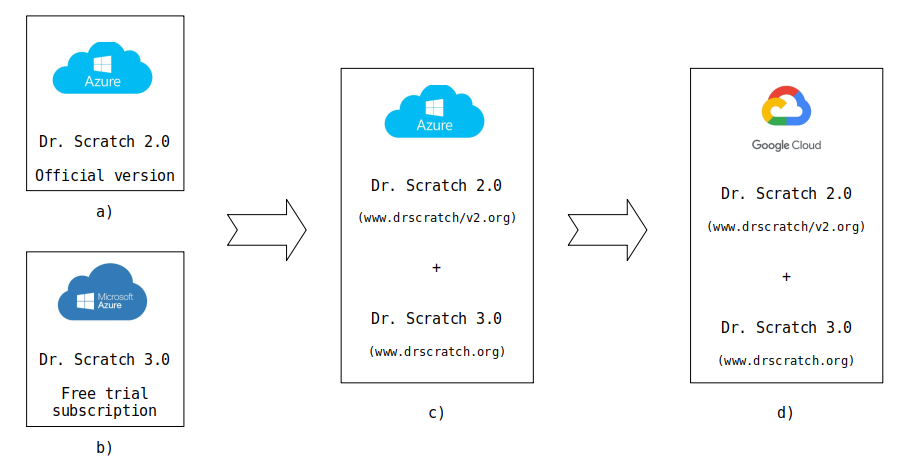
\includegraphics[width=14cm, keepaspectratio]{img/migrations.png}
    \caption{Migration process for the new version of Dr. Scratch.}
    \label{fig:migrations}
\end{figure}


Thanks to an educational subscription, we had a free trial period of the services offered by Azure during a month. In this way, we configured a virtual machine with the new version of Dr. Scratch and we tested it during a month, as we can observe in Figure~\ref{fig:migrations} b). To carry out this process, it was necessary to configure Apache throughout the file \textit{httpd.conf}. This file contained the instructions for the main settings. In addition, we needed a testing database with MySQL.

After correcting some small errors during the trial period, such as the download of certificates or the change of language,  we configured the official virtual machine of Azure with both versions of Dr. Scratch, as we observe in Figure~\ref{fig:migrations} c). Again, it was possible thanks to the configuration of the \textit{httpd.conf} file of Apache. 

Finally, in January 2019 we launched the new version. Dr. Scratch 3.0 was allocated in the \textit{www.drscratch.org} domain. Its main page contained a link which redirected to the old version, allocated in the \textit{www.drscratch.org/v2} domain. We can observe the main interface of the tool in Figure~\ref{fig:dr_scratch}.


\subsection{Migration of Dr. Scratch 3.0 to Google Cloud Platform}
\label{subsec:mig_to_google}

In April 2019, the funding which we received from Microsoft was over and we studied different options to allocate Dr. Scratch. Finally, the best solution found was to migrate the application to the Google Cloud technology, as we can observe in Figure~\ref{fig:migrations} d).
 
We received a grant from the GCP Research and, thanks to that, we configured the new services. We deployed a new virtual machine with 18.04.4 Linux as operative system. In addition, we updated MySQL to the 5.7.28 version. We migrated both versions to the new platform and we configured again the Apache module. It was a quick process and we had a short trial period. After solving small problems, we got a stable version which is working at present.


\section{Analysis of bad smells}
\label{sec:analysis}

Despite the new version Dr. Scratch 3.0 was stable in the Google Cloud Platform, all the analysis of bad smells was carried out with Dr. Scratch 2.0. The reason was that the data set used in the analysis was composed of projects designed with the old version of Scratch, that is, with the \textit{.sb2} extension and its corresponding format.

Therefore, both data sets were analyzed with the Hairball module of Dr. Scratch 2.0. The Dr. Scratch tool in the previous version identified four different types of bad smells that can be present in Scratch projects~\cite{robles2017software}: copy and pasted code (duplicate scripts), the use of default names for sprites (default names), code that is never being executed (dead code), and variables that are not correctly initialized (attribute initialization).

Their description and characteristics, as well as their impact in the CT development, are summarized in Table~\ref{table:bad_smells}.

\begin{table}
 \begin{center}
  \begin{tabular}{|p{4cm}|p{5cm}|p{5cm}|}
    \hline
    \textbf{Bad Smell Type} & \textbf{Definition} & \textbf{Impact on Learning} \\ \hline
    \textbf{Duplicated scripts} & Code is copy and pasted, sometimes with minor changes & It hinders the use of user-defined blocks and as such can be seen a limitation to the development of the abstraction skill \\ \hline
    \textbf{Default names} & Objects are not given a meaningful name, but keep the default {\em SpriteN} name & It hinders interaction among objects, as using them in other objects becomes more difficult \\ \hline
    \textbf{Dead code} & Code that is never being executed (usually because they do not have a starting condition) & It may indicate missing functionality \\ \hline
    \textbf{Attribute initialization} & Variables are not well initialized & It hinders the start of some objects, because their position, size or costume, among others, are not correctly initialized \\ \hline
  \end{tabular}
  \caption{Description of bad smells and their impact on learning.}
  \label{table:bad_smells}
 \end{center}
\end{table}

\subsection{Data set description}
\label{subsec:descrip_dataset}

In order to analyze the presence of bad smells, as well as their relationship with the level that users have in CT development, a large set of projects was necessary. In this work we have analyzed two different data set. The first of them, which we will call data set a, was analyzed in a preliminary and general analysis. In order to improve and verify the results obtained, we repeated the analysis with a bigger data set, which we will call data set b. The distribution of both data set is summarized in Table~\ref{table:dataset_distribution}.

\begin{table}
 \begin{center}
  \begin{tabular}{|c|c|c|}
    \hline
    & \textbf{Number of projects} & \textbf{Number of snapshots} \\ \hline
    \textbf{Data set a} & 771 & 62,074 \\ \hline
    \textbf{Data set b} & 250,163 & - \\ \hline
  \end{tabular}
  \caption{Distribution of the data set used in the general preliminary analysis.}
  \label{table:dataset_distribution}
 \end{center}
\end{table}


\subsubsection{Data set a}
\label{subsubsec:dataset_a}

Data set a was created and studied in another, previous research~\cite{troiano2019my}. A group of 438 students designed games for STEM using Scratch 2.0. During this process, the authors obtained snapshots of the process each minute during a period of time -only if the project registered changes-, in order to show a timeline evolution. The total number of projects without taking into account the replicas over time, was 771. The total number of snapshots over time were 62,074, with an average of 78 snapshots per project.

As a result, the complete data set was comprised of 62,074 samples formed by the different snapshots of each project\footnote{https://drive.google.com/drive/u/0/folders/1tDI6nx2f6344xJAKeUeWBeTg0YzxE3bO}. The objective of storing snapshots was to analyze the same 771 projects in different points of time.

\subsubsection{Data set b}
\label{subsubsec:dataser_b}

Data set b was also created and analyzed in another previous research~\cite{aivaloglou2017dataset}. This data set contained 250,163 Scratch projects, from more than 100,000 different users of its community. These projects were scraped from the Scratch repository. The scraper and all the project files are available in the GitHub repository \textit{TU Delft Scratch Research Team}\footnote{https://github.com/TUDelftScratchLab/ScratchDataset}.

From this repository, we stored the useful data in two CSV files, \textit{metadata.csv} and \textit{code.csv}. These files included, for each Scratch project, its metadata -user name, total views or the project URL, among others- and information about its code -sprite types, block types, total blocks or CT development of the Dr. Scratch assessment, among others-, respectively.


\subsection{Data collection}
\label{subsec:datacollection}

From this point, we needed to create our own CSV files from the data set described above. The process of the data set construction for the analysis is detailed below.

\subsubsection{Data set a}
\label{subsubsec:datacollection_a}

In order to analyze the 62,074 snapshots with the Dr. Scratch tool, it was necessary to design a script. This script, \textit{projects\_analyzer.py}, was programmed in Python. Its main function was to open each folder with the Scratch project and analyze its JSON file. As we mentioned previously, the analysis was carried out with the Hairball module and all its plugins. The result obtained from the script was a CSV file, \textit{evolution\_time\_results.csv}, with the information necessary for the analysis: the total mastery, the score of each category of the CT, data about bad smells and data about the blocks.

During the analysis process, we found 2,158 erroneous snapshots due to different reasons: the project was saved incorrectly, the code contained special characters or some field was empty, among others. In this way, the final set of valid samples for the analysis was comprised of 59,916 snapshots and 754 projects.

On the other hand, we programmed another script to analyze the latest registered version of each project. In other words, we designed a script which analyzed the 771 projects without the timeline evolution. The result obtained was another CSV file, \textit{final\_projects\_results.csv}, with the same structure than \textit{evolution\_time\_results.csv}, but storing only the last snapshot of each project. Again, we found the same erroneous samples and the final valid data set was comprised of 754 projects.

The statistics and distribution of valid projects and snapshots for the analysis are summarized in Table~\ref{table:datacollection_a}.

\begin{table}
 \begin{center}
  \begin{tabular}{|c|c|c|c|c|}
    \hline
     & \textbf{Total samples} & \textbf{Valid samples} & \textbf{Wrong samples} & \textbf{Survival ratio} \\ \hline
    \textbf{Projects} & 771 & 754 & 17 & 97.80\% \\ \hline
    \textbf{Snapshots}& 62,074 & 59,916 & 2,158 & 96.52\% \\ \hline
  \end{tabular}
  \caption{Distribution of the final data set a used in the general analysis.}
  \label{table:datacollection_a}
 \end{center}
\end{table}


\subsubsection{Data set b}
\label{subsubsec:datacollection_b}

The size of the data set b was much bigger than the data set a. For this reason, we found complications when we tried to open the file \textit{code.csv} and analyze it. Its analysis with a Python script was too slow and required too much storage space.

Finally, the solution was to create a Jupyter notebook and read and analyze the file line by line. In this way, we could join and select the useful information from the \textit{code.csv} and \textit{metadata.csv} files. The result of the Jupyter notebook was a new CSV file, \textit{final\_dataset.csv}, composed of the useful data from both files and with the structure which we wanted for the analysis: total mastery, the score of each category of CT and information about bad smells and the blocks. 

During the analysis process, we found wrong projects again. We found null data in the \textit{metadata.csv} file and special characters in the \textit{code.csv}. Finally, the number of valid projects was 231,024. The statistics of the valid samples for the data set b are summarized in Table~\ref{table:datacollection_b}.

\begin{table}
 \begin{center}
  \begin{tabular}{|c|c|c|c|c|}
    \hline
     & \textbf{Total samples} & \textbf{Valid samples} & \textbf{Wrong samples} & \textbf{Survival ratio} \\ \hline
    \textbf{Projects} & 250,163 & 231,024 & 19,139 & 92.35\% \\ \hline
  \end{tabular}
  \caption{Distribution of the final data set b used in the general analysis.}
  \label{table:datacollection_b}
 \end{center}
\end{table}
    

\subsection{General analysis}
\label{subsec:generalanalysis}

The main objective of this phase was to analyze the presence of several bad smells in Scratch projects and how they relate to the development of CT skills. We carried out a preliminary analysis with the data set a in order to analyze to what extent bad smells are present in Scratch projects and what is its impact. Then, we repeated the same analysis with data set b in order to verify the results with a bigger set of projects. We developed both analysis with Jupyter notebook, based on the CSV files generated in the previous section. 

The starting point of the general analysis was to raise the main research questions that we wanted to analyze. All the proposal, as well as the development of the analysis and the results obtained, were published in the paper ``Bad Smells in Scratch Projects: A Preliminary Analysis''~\cite{vargas2019bad}. We developed this paper for the EC-TEL congress\footnote{http://www.ec-tel.eu/} and we presented it in the TACKLE workshop\footnote{https://sites.google.com/site/2019tackleworkshop/home} (the 2nd Systems of Assessments for Computational Thinking Learning) in Delft, Netherlands.

\subsubsection{RQ1. To what extent are bad habits present in Scratch projects?}
\label{subsubsec:RQ1}

In particular, we answer this question by offering the percentage of projects that have at least one type of bad smell. This question allows to see how frequent projects show a bad smell, hinting to the relevance of the topic. We expect a significant number of projects to contain bad smells.

\subsubsection{RQ2. Does the development of CT skills relate to a minor presence of bad smells?}
\label{subsubsec:RQ2}

We would like to find out if the presence of bad smells correlates with the complexity of the projects. Our hypothesis is that projects that have higher degrees of CT development will have less bad smells, as these may hinder the development of CT skills.

\subsubsection{RQ3. Do projects with more blocks have a higher number of bad smells?}
\label{subsubsec:RQ3}

More complex projects usually have more blocks. Thus having a single bad smell in a small, simple project may have less impact than in a project with hundreds of blocks. In the former case, the impact could be big, while in the latter it could be seen as an exception, with little impact.

To answer this question, for projects of the same level of CT development we calculate the ratio of the number of bad smells detected to the total number of blocks. We expect that this ratio decreases with an increase in the development of CT skills required to create the Scratch projects.

\subsubsection{RQ4. Can we find a relation among specific bad smells?}
\label{subsubsec:RQ4}

As by now, we have considered all type of bad smells together. In this question, we dig into each of them separately. It may be possible that some bad smells appear more frequently in projects of lower complexity, while others appear in more complex projects.

\subsubsection{RQ5. To which extent can bad smells be identified in each of the CT development phases?}
\label{subsubsec:RQ5}

Related to the previous question, we analyze how the different bad smell types appear in projects in the different stages of CT development. Therefore, we consider projects with a low complexity (basic), medium complexity (developing) and major complexity (proficiency) and compute how often they contain a specific type of bad smell.

We expect that several types of bad smells appear in the early phases (basic), while others are more prominent in more complex projects (proficiency). We assume therefore that learners that achieve higher levels of complexity have overcome certain bad smells due to having developed certain CT skills, while other bad smells appear in those more complex projects.


\subsection{Statistical analysis}
\label{subsec:statisticalanalysis}

After the general preliminary analysis, we decided to deepen the study and develop a more specific analysis. In order to analyze in more detail the impact of bad smells in our variable of interest (CT development), we carried out a statistical analysis. The main objectives of this analysis were: 

\begin{itemize}
    \item To analyze the behaviour and distribution of each type of bad smell through Dr. Scratch, during the timeline of the projects.
    \item To analyze the impact on the development of the CT skills.
    \item To carry out a statistical \textit{t-student} study in order to measure the effect that bad smells have throughout a period of time. 
\end{itemize}

In order to develop these objectives, we compared two main groups or populations. The first of them was a set of projects with a few amount of bad smells and the other one, a set of projects with a huge amount of bad smells, in a given initial state. Afterwards, we wanted to know if they showed a different timeline evolution.

From this point, there were two hypotheses, \textit{H0} -both populations presented no differences in the mean value of bad smells- and \textit{H1} -the populations had different mean value of bad smells. We wanted to prove how random could be \textit{H1}.   


\subsubsection{Sample processing}
\label{subsubsec:sample_processing}

Therefore, this second study was based on data set a, since it was necessary a timeline evolution of the projects. To perform an effective analysis, we divided the total number of snapshots into deciles, that is, into 10 proportional periods of time (D0-D9), for each project. Afterwards, only those projects with at least 10 snapshots -at least one snapshot per decile- were considered as valid samples. In addition, we also removed those projects which had 0 points in the assessment with Dr. Scratch in D9. These projects did not have any development, so they were not useful for the study. 

The final data set after removing invalid and null samples was composed of 543 projects and 59,332 snapshots. The survival ratio about valid projects decreases considerably due to a high density of projects with less than 10 registered snapshots. We can observe this effect in Figure~\ref{fig:distribution_snapshots_deciles}. Its distribution is also shown in Table~\ref{table:statistical_analysis_distribution_samples}. 

The distribution of the snapshots, for both participating projects and valid projects, is described, in a more detailed way, in Table~\ref{table:statistical_analysis_distribution_snapshots}.

Finally, in order to avoid redundant information, we only stored the last registered snapshot of each project, in each decile. In this way, the data set for the analysis was composed of 543 projects and 5430 snapshots, with only one snapshot per decile.


\begin{table}
    \centering
    \begin{tabular}{|c|c|c|c|}
        \hline
        & \textbf{Total samples} & \textbf{Valid samples} & \textbf{Survival ratio} \\ \hline
        \textbf{Projects} & 754 & 543 & 72.02\% \\ \hline
        \textbf{Snapshots} & 59,915 & 59,332 & 99.03\% \\ \hline
    \end{tabular}
    \caption{Distribution of the processed data set for the statistical analysis with deciles.}
    \label{table:statistical_analysis_distribution_samples}
\end{table}

\begin{table}
    \centering
    \begin{tabular}{|c|c|c|c|c|}
        \hline
        & \textbf{Minimal number} & \textbf{Maximum number} & \textbf{Mean} &\textbf{Standard} \\
        & \textbf{of snapshots} & \textbf{of snapshots} & \textbf{of snapshots} & \textbf{deviation} \\ \hline
        \textbf{Participating projects} & 0 & 597 & 78.0 & 82.1 \\ \hline
        \textbf{Valid projects} & 11 & 597 & 109.3 & 77.8 \\ \hline
    \end{tabular}
    \caption{Snapshot distribution in the processed data set for the statistical analysis with deciles.}
    \label{table:statistical_analysis_distribution_snapshots}
\end{table}

\begin{figure}
  \centering
  \begin{subfigure}{9cm}
    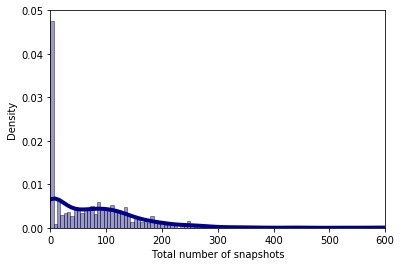
\includegraphics[width=9cm]{img/snapshots_participant_projects.png}
    \caption{Participant projects}
    \label{subfig:participant_projects}
  \end{subfigure}
  \begin{subfigure}{9cm}
    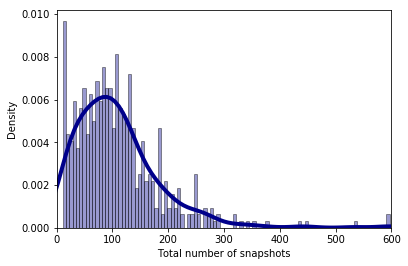
\includegraphics[width=9cm]{img/snapshots_valid_projects.png}
    \caption{Valid projects}
    \label{subfig:valid_projects}
  \end{subfigure}
  \caption{Snapshot distribution for the statistical analysis with deciles.}
  \label{fig:distribution_snapshots_deciles}
\end{figure} 


\subsubsection{Characteristics of the sample}
\label{subsubsec:sample_distribution}

After dividing the valid data set into deciles, we analyzed its distribution according to the CT development obtained in the assessment with the Dr. Scratch tool. In Table~\ref{table:ct_development_deciles} is summarized this information for D0 and D9, in order to show the evolution between the initial and final state of the projects.

We can observe how the density of the projects with a higher CT development is bigger in D9 than in D0. On the contrary, the density of projects with a lower CT development is bigger in D0 than in D9. This distribution implies a CT development throughout the timeline of the projects. We can observe this effect in a more visual way in Figure~\ref{fig:ct_development}. 

\begin{table}
    \centering
    \begin{tabular}{|c|c|c|c|c|}
        \hline
        \textbf{Dr. Scratch CT} & \multicolumn{2}{|c|}{\textbf{Frequency}} & \multicolumn{2}{|c|}{\textbf{Percent (\%)}} \\ \cline{2-5}
        \textbf{Assessment} & \textbf{D0} & \textbf{D9} & \textbf{D0} & \textbf{D9}   \\ \hline 
        0 & 46 & 0 & 8.47 & 0.00 \\ \hline
        1 & 10 & 0 & 1.84 & 0.00 \\ \hline
        2 & 8 & 1 & 1.47 & 0.18 \\ \hline
        3 & 18 & 1 & 3.31 & 0.18 \\ \hline
        4 & 16 & 1 & 2.95 & 0.18 \\ \hline
        5 & 41 & 6 & 7.55 & 1.10 \\ \hline
        6 & 28 & 3 & 5.16 & 0.55 \\ \hline
        7 & 20 & 17 & 3.68 & 3.13 \\ \hline
        8 & 44 & 12 & 8.10 & 2.21 \\ \hline
        9 & 34 & 11 & 6.26 & 2.03 \\ \hline
        10 & 43 & 14 & 7.92 & 2.58 \\ \hline
        11 & 54 & 33 & 9.94 & 6.08 \\ \hline
        12 & 43 & 45 & 7.92 & 8.29 \\ \hline
        13 & 35 & 58 & 6.45 & 10.68 \\ \hline
        14 & 36 & 114 & 6.63 & 20.99 \\ \hline
        15 & 19 & 59 & 3.50 & 10.87 \\ \hline
        16 & 26 & 69 & 4.79 & 12.71 \\ \hline
        17 & 11 & 44 & 2.03 & 8.10 \\ \hline
        18 & 3 & 25 & 0.55 & 4.60 \\ \hline
        19 & 3 & 22 & 0.55 & 4.05 \\ \hline
        20 & 5 & 6 & 0.92 & 1.10 \\ \hline
        21 & 0 & 2 & 0.00 & 0.37 \\ \hline
        \textbf{Total} & \multicolumn{2}{|c|}{\textbf{543}} & \multicolumn{2}{|c|}{\textbf{100}} \\ \hline
    \end{tabular}
    \caption{Distribution of the CT development for the valid data set in D0 and D9.}
    \label{table:ct_development_deciles}
\end{table}

\begin{figure}
    \centering
    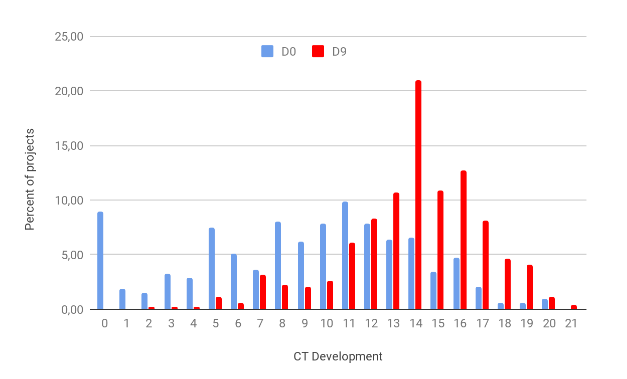
\includegraphics[width=12cm,                         keepaspectratio]{img/CT_development.png}
    \caption{Distribution of the CT development for the valid data set in D0 and D9.}
    \label{fig:ct_development}
\end{figure}

On the other hand, we also analyzed the distribution of the number of bad smells in each decile. In Figure~\ref{fig:bad_smells_deciles} is shown the mean value of each bad smell for each decile. As we can observe, the number of bad smells increases with the timeline evolution. This result could be produced by the increase of the CT development of the projects and, consequently, with the increase of its number of blocks.

\begin{figure}
    \centering
    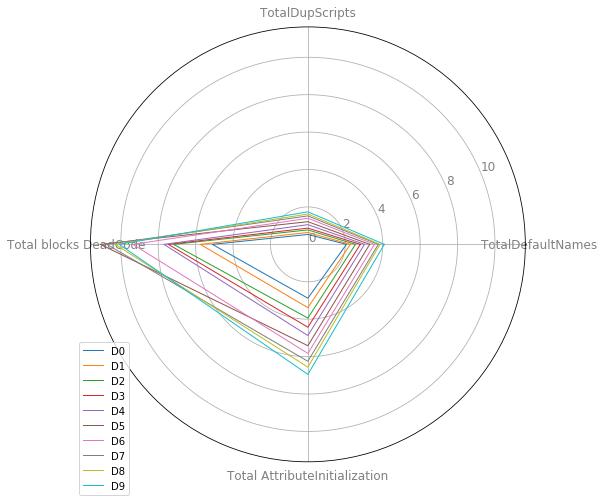
\includegraphics[width=11cm,                         keepaspectratio]{img/bad_smells_deciles.png}
    \caption{Distribution of the mean value of each bad smell for the deciles D0-D9.}
    \label{fig:bad_smells_deciles}
\end{figure}

In order to verify this effect, we analyzed the ratio between the mean value of each bad smell and the total number of blocks in the projects, for each decile. In this way, we obtained the contrary effect, as we can observe in Figure~\ref{fig:ratio_bad_smells_deciles}. In this figure, the ratio decreases with each decile. In other words, the mean value of bad smells is lower when the CT development increases, as we expected. 

\begin{figure}
    \centering
    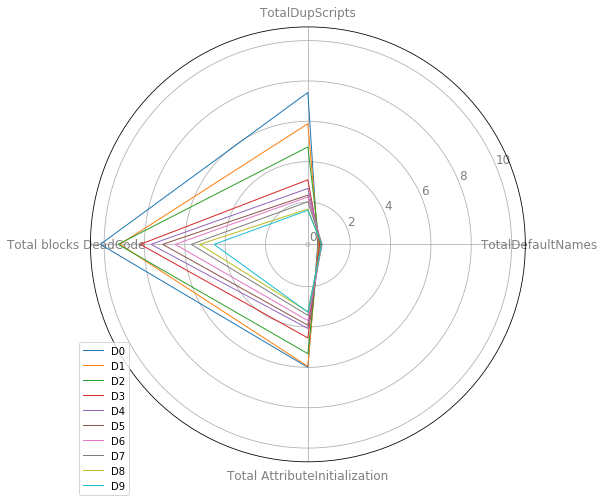
\includegraphics[width=11cm,                         keepaspectratio]{img/ratio_bad_smells_deciles.png}
    \caption{Mean value of each bad smell / Total number of blocks (\%) for the deciles D0-D9.}
    \label{fig:ratio_bad_smells_deciles}
\end{figure}

\subsubsection{\textit{T-student} test}
\label{subsubsec:test_tstudent}

After analyzing the distribution and the characteristics of the data set, we found that the main development was more prominent from the decile D2. Therefore, the most effective populations for the study were in D2 and D9, as the final state. 

From this point, we investigated the most appropriate procedure to develop the statistical analysis. It was the \textit{t-student} test, which compares the measures obtained -the mean value of bad smells- in two different groups for a given variable, the CT development.

This test allows us to know the probability to obtain results just by chance. If the probability is high, we can say that the results are due to randomness. On the contrary, if the probability is low, we can say that the differences obtained in the test are probably real. In other words, with a low probability we could reject \textit{H0} -both populations do not present differences in the mean value of bad smells. 

The variable which we used in the analysis to measure this probability was the \textit{p-value}. By agreement, it is established that a \textit{p-value} less than 0.05 indicates that the result of the analysis is not random and \textit{H0} can be reasonably rejected. Therefore, if the \textit{p-value} is greater than 5\%, we cannot affirm that the differences in the results are reliable.  

In addition, we calculated the \textit{size effect} for each test. This variable measures the magnitude of the effect studied. In other words, if we find differences in the results, we want to measure how is the size of these differences. A value greater than 0.5 indicates that the \textit{size effect} is `large' and the differences are significant.

\subsubsection{Development of the statistical analysis}
\label{subsubsec:development_statistical_analysis}

After the treatment and analysis of the data set and the choice of the \textit{t-student} test, we developed the study with Jupyter notebook. In particular, we implemented the function \textit{ttest\_ind}, which calculates the \textit{t-student} test for the value of two independent groups. For the computation of the \textit{size effect}, we used an automatic online calculator\footnote{https://www.psychometrica.de/effect\_size.html}. 

\hfill

{\footnotesize
\begin{verbatim}
    scipy.stats.ttest_ind(population_a, population_b, equal_var=False)
\end{verbatim}
}

\hfill

With this function we obtained the \textit{p-value} -we assumed that the populations had no identical variances.

From this point, we carried out the \textit{t-student} test for different populations in order to find reliable results. We describe each case of study as a research question.


\subsubsection{RQ1. \textit{T-student} test with deciles}
\label{subsubsec:rq1_t_student_deciles}

In the first place, we carried out an analysis with two general groups. The first of them was composed of a set of projects in D9 which had a few bad smells in D2. The other one was a set of projects in D9 which had many bad smells in D2. 

With this research question we wanted to verify if the population A could present a minor mean value of bad smells in D9 than population B and, in that case, if the differences would be reliable -in terms of \textit{p-value} and \textit{size effect}. In this way, the populations were the following:

\begin{itemize}
    \item[--] Population A: Projects in D9 which had less than 5 bad smells in D2 (N=168).
    \item[--] Population B: Projects in D9 which had more than 20 bad smells in D2 (N=95).
\end{itemize}


\subsubsection{RQ2. \textit{T-student} test with deciles for a given CT development}
\label{subsubsec:rq2_t_student_deciles_ct}

One of the objectives of this analysis was to measure the impact of bad smells in the CT development. In RQ1, we found significant differences in the level of CT between the two groups of study, as we will describe in Chapter~\ref{chap:results}. For this reason, we repeated the \textit{t-student} test, but based on a specific set of projects of the data set. 

We selected those projects whose CT development obtained with Dr. Scratch in D2 was included in the interval [7,12) points of mastery. The objective of this study was to enclose the populations in projects with similar CT development and compare them.

Finally, the total number of this data set was 184 projects and we chose the same populations.

\begin{itemize}
    \item[--] Population A: Projects in D9 which had less than 5 bad smells in D2 (N=62).
    \item[--] Population B: Projects in D9 which had more than 20 bad smells in D2 (N=21).
\end{itemize}


\subsubsection{RQ3. \textit{T-student} test without deciles}
\label{subsubsec:rq3_t_student_no_deciles}

We found very significant results both in RQ1 and RQ2, as we will describe in more detail in Chapter~\ref{chap:results}. However, we realized that we were comparing very similar projects in each decile and the analysis was not reliable. In addition, we found in the results a very alarming fact: Dr. Scratch tool could assess positively the presence of bad smells. 

Therefore, we repeated the \textit{t-student} test with another proposal. In this case, we selected only two snapshots for each project: the first snapshot in which the project got 7 points of CT development, and the last snapshot of the project. We call each situation as D0 and D1, respectively.

\begin{itemize}
    \item[--] D0: The first snapshot in which the project gets 7 points in the CT development, measured with Dr. Scratch. 
    \item[--] D1: The last snapshot of each project in D0.
\end{itemize}

The data set extracted consisted of 452 snapshots, divided in 226 snapshots for each population. This distribution is summarized in Table~\ref{table:distribution_without_deciles}. Based on these groups, we developed different analysis.

\begin{table}
    \centering
    \begin{tabular}{|c|c|c|}
        \hline
        \textbf{Total samples} & \textbf{Samples in D0} & \textbf{Samples in D1} \\ \hline
        452 & 226 & 226 \\ \hline
    \end{tabular}
    \caption{Description of the data set used in the statistical analysis without deciles.}
    \label{table:distribution_without_deciles}
\end{table}

\subsubsection{RQ3.1. \textit{T-student} test without deciles for the total number of bad smells}
\label{subsubsec:RQ3_1_statistical}

The first research question was carried out with the total number of bad smells, that is, the sum of each type of bad smell. With this analysis, we wanted to verify the same concepts than in RQ1. We selected two populations and developed again the \textit{t-student} test.

\begin{itemize}
    \item[--] Population A: Projects in D1 which had less than 5 bad smells in D0 (N=129).
    \item[--] Population B: Projects in D1 which had more than 20 bad smells in D0 (N=11).
\end{itemize}


\subsubsection{RQ3.2. \textit{T-student} test without deciles for default naming}
\label{subsubsec:RQ3_2_statistical}

We repeated the \textit{t-student} test for each bad smell independently, in order to avoid the noise introduced by the sum of all of them.

In addition, we selected several cases of study for each analysis by modifying the percentage of the population B. We started with a low percent in case 1 and we increased it in each case. In other words, we wanted to show the differences in the evolution based on different percents of bad smells in population B.

\begin{itemize}
    \item[--] Case 1
    \begin{enumerate}[(i)]
        \item Population A: Projects in D1 which had 0\% of default names over the total number of sprites in D0 (N=137).
        \item Population B: Projects in D1 which had more than 30\% of default names over the total number of sprites  in D0 (N=64).
    \end{enumerate}
    \item[--] Case 2
    \begin{enumerate}[(i)]
        \item Population A: Projects in D1 which had 0\% of default names over the total number of sprites in D0 (N=137).
        \item Population B: Projects in D1 which had more than 50\% of default names over the total number of sprites  in D0 (N=30).
    \end{enumerate}
    \item[--] Case 3
    \begin{enumerate}[(i)]
        \item Population A: Projects in D1 which had 0\% of default names over the total number of sprites in D0 (N=137).
        \item Population B: Projects in D1 which had more than 70\% of default names over the total number of sprites  in D0 (N=24).
    \end{enumerate}
    \item[--] Case 4
    \begin{enumerate}[(i)]
        \item Population A: Projects in D1 which had 0\% of default names over the total number of sprites in D0 (N=137).
        \item Population B: Projects in D1 which had more than 100\% of default names over the total number of sprites in D0 (N=22).
    \end{enumerate}
\end{itemize}


\subsubsection{RQ3.3. \textit{T-student} test without deciles for duplicated code}
\label{subsubsec:RQ3_3_statistical}

The data set composed of projects with duplicated code was too small. For that reason, we only selected one case of study with the following populations. 

\begin{itemize}
    \item[--] Population A: Projects in D1 which had not duplicated code in D0 (N=217).
    \item[--] Population B: Projects in D1 which had at least 1 duplicated code in D0 (N=9).
\end{itemize}


\subsubsection{RQ3.4. \textit{T-student} test without deciles for dead code}
\label{subsubsec:RQ3_4_statistical}

For the statistical analysis of the dead code, we selected three different cases of study, described below.

\begin{itemize}
    \item[--] Case 1
    \begin{enumerate}[(i)]
        \item Population A: Projects in D1 which had 0\% of dead code over the total blocks in D0 (N=116).
        \item Population B: Projects in D1 which had more than 20\% of dead code over the total blocks in D0 (N=73).
    \end{enumerate}
    \item[--] Case 2
    \begin{enumerate}[(i)]
        \item Population A: Projects in D1 which had 0\% of dead code over the total blocks in D0 (N=116).
        \item Population B: Projects in D1 which had more than 30\% of dead code over the total blocks in D0 (N=55).
    \end{enumerate}
    \item[--] Case 3
    \begin{enumerate}[(i)]
        \item Population A: Projects in D1 which had 0\% of dead code over the total blocks in D0 (N=116).
        \item Population B: Projects in D1 which had more than 50\% of dead code over the total blocks in D0 (N=28).
    \end{enumerate}
\end{itemize}



\subsubsection{RQ3.5. \textit{T-student} test without deciles for attribute initialization}
\label{subsubsec:RQ3_5_statistical}

Finally, the last research question was carried out for the attribute initialization. In this case, we selected two different situations for the analysis. 

\begin{itemize}
    \item[--] Case 1
    \begin{enumerate}[(i)]
        \item Population A: Projects in D1 which had 0\% of attribute initialization over the total blocks in D0 (N=68).
        \item Population B: Projects in D1 which had more than 20\% of attribute initialization over the total blocks in D0 (N=15).
    \end{enumerate}
    \item[--] Case 2
    \begin{enumerate}[(i)]
        \item Population A: Projects in D1 which had 0\% of attribute initialization over the total blocks in D0 (N=68).
        \item Population B: Projects in D1 which had more than 30\% of attribute initialization over the total blocks in D0 (N=6).
    \end{enumerate}
\end{itemize}


\section{Bad smells model}
\label{sec:badsmells}

After the development of the full analysis, we discovered that the presence of bad smells in the Scratch projects was very significant, as well as its effect on the CT development. All the results will be detailed in Chapter~\ref{chap:results}. 

From this point, we considered necessary to develop a new environment in the Dr. Scratch tool, in order to show in the first place the results about bad smells and raise awareness about them. We will call this new environment bad smells model. 

As we described in Section~\ref{sec:reference}, the dashboard of bad smells in the Dr. Scratch interface was very small and hard to interpret. Therefore, the main objective of this phase was to replace the dashboards, shown in Figure~\ref{fig:dashboards}, by the new model with more visual information about bad smells, shown in Figure~\ref{fig:bad_smells_model}. The process of developing the bad smells model was composed of different phases.

\subsection{\textit{Scratchblocks} library}
\label{subsec:scratchblocks}

The dashboard of bad smells showed the information with text format. In this way, it was more difficult to understand the presence of bad smells in the projects and, consequently, to interpret this information and correct them. Therefore, the starting point was to replace the dashboard with the text by visual blocks.

The \textit{scratchblocks} library\footnote{https://github.com/scratchblocks/scratchblocks} makes pictures of Scratch blocks from text. We included this library in the code of Dr. Scratch and created a new template with four dashboards, one for each bad smell. In addition, we programmed a new script, \textit{sb3\_blocks\_mapper.py}, to map the name of the blocks from the JSON file to the \textit{scratchblocks} library.

From this point, we found the problem that the scripts developed in the Phase 1 of this project returned the information about bad smells in a format which \textit{sb3\_blocks\_mapper.py} could not interpret. Therefore, we had to change some functionalities in each script.


\subsection{Improvement of the scripts}
\label{subsec:improvement_scripts}

The scripts which we developed in the Phase 1 of the project were designed to return the information in a text list. For this reason, we had to change the code of all of them and to adapt the list of results of each bad smell to the new format.

In addition, in order to show the results in an easier way to interpret, we added new functionalities, detailed below:

\begin{itemize}
    \item[--] Sprite naming: detection of default naming for more languages (Personatge, Figura, O actor, Personaia).
    \item[--] Backdrop naming: detection of default naming for more languages (Fons, Atzeko oihala).
    \item[--] Dead code: differentiation of dead code for each sprite, shown in Figure~\ref{fig:dead_code}.
    \item[--] Duplicated code: differentiation and identification of the sprites who have the duplicated blocks, shown in Figure~\ref{fig:dup_code}.
\end{itemize}

\begin{figure}
    \centering
    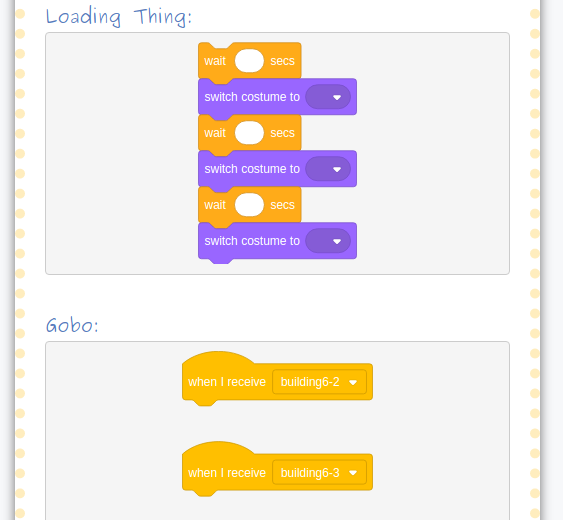
\includegraphics[width=9cm,                         keepaspectratio]{img/dead_code.png}
    \caption{Example of the dead code dashboard for different sprites in the bad smells mode.}
    \label{fig:dead_code}
\end{figure}

\begin{figure}
    \centering
    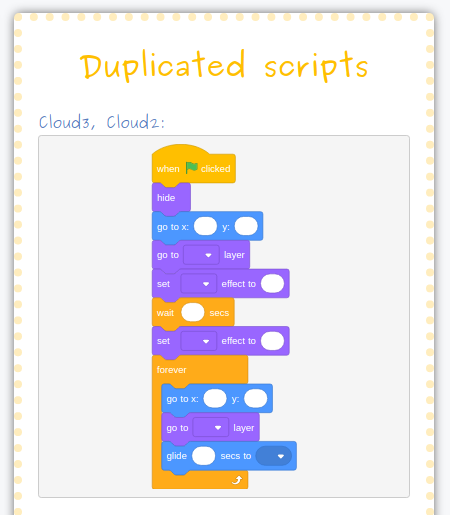
\includegraphics[width=9cm,                         keepaspectratio]{img/dup_code.png}
    \caption{Example of the duplicated code dashboard for two sprites in the bad smells mode.}
    \label{fig:dup_code}
\end{figure}


\subsection{Integration of the bad smells model in Dr. Scratch}
\label{subsec:integration_newmodel}

The last step for the development of the bad smells model was its integration in the Dr. Scratch code. When users analyzed a Scratch project with Dr. Scratch, they received the response with all the dashboards. We replaced this template for the template with the new model, which can be observed in Figure~\ref{fig:newmodel}.

\begin{figure}
    \centering
    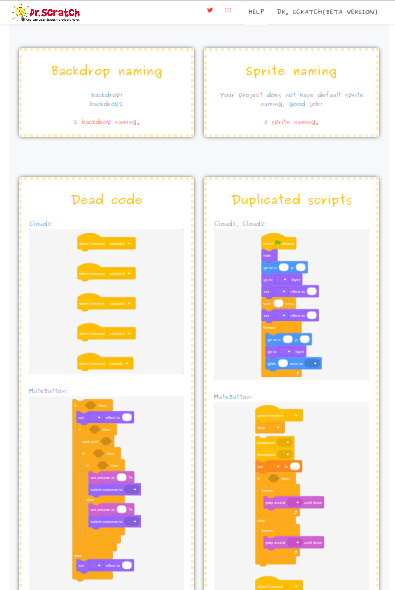
\includegraphics[width=12cm,                         keepaspectratio]{img/newmodel.png}
    \caption{New interface of Dr. Scratch for the bad smells model.}
    \label{fig:newmodel}
\end{figure}

In addition, we added a new button to access the old dashboards. In other words, once that users have analyzed their results about bad smells, they can navigate to the rest of dashboards with the CT development results and the download of the certificate. We can observe this functionality in Figure~\ref{fig:button}.

\begin{figure}
    \centering
    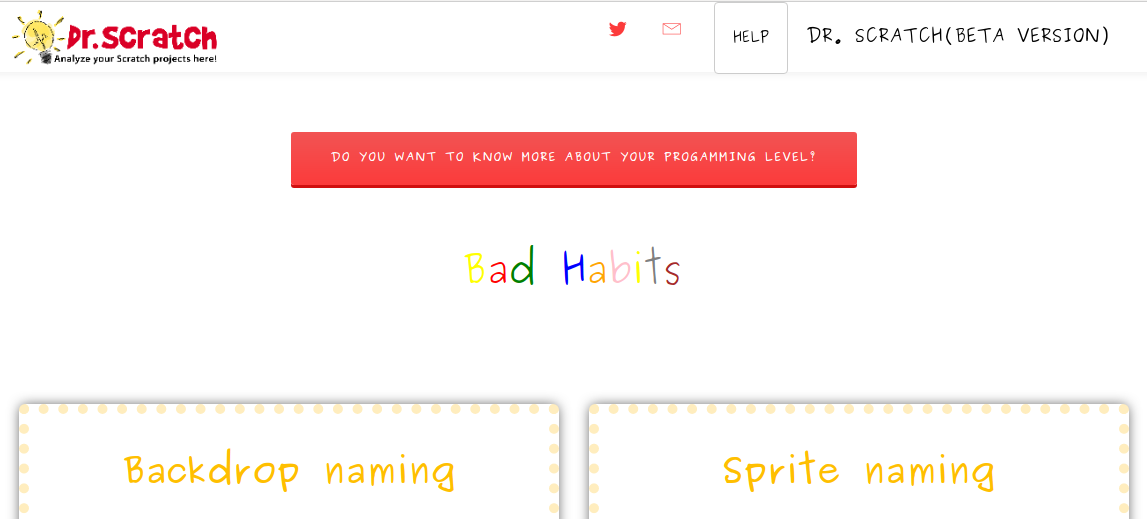
\includegraphics[width=11cm,                         keepaspectratio]{img/button.png}
    \caption{Button in the bad smells model to access the rest of the dashboards.}
    \label{fig:button}
\end{figure}


Finally, when the user profile was basic (from 0 to 7 points), the Dr. Scratch tool did not show the dashboard with the information about bad smells. Users who are beginning do not need all this information. For this reason, we though that it was better to avoid the bad smells model for this type of users. When the total mastery is less than seven points, Dr. Scratch shows the normal dashboards instead of the bad smells model, as we can observe in Figure~\ref{fig:basic_level}.

\begin{figure}
    \centering
    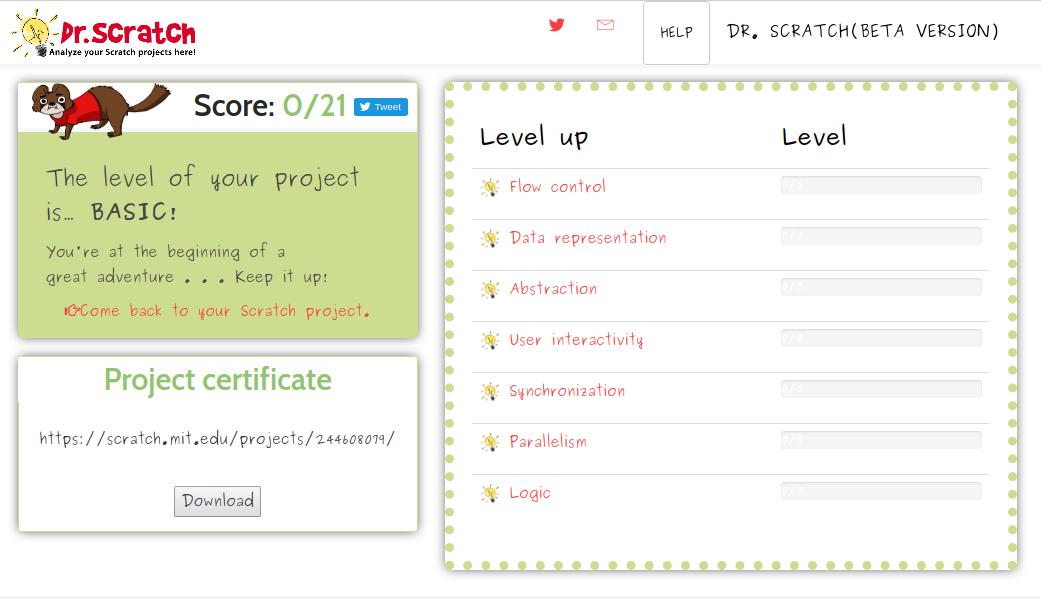
\includegraphics[width=11cm,                         keepaspectratio]{img/basic_level.png}
    \caption{Interface of Dr. Scratch for users with Basic profile.}
    \label{fig:basic_level}
\end{figure}


\section{Assessment experiment}
\label{sec:experiment}

After the development of the bad smells model and its implementation, we wanted to verify the effectiveness of our study as the last phase of the project. To do this, we designed an assessment experiment in which two teachers -without any knowledge about bad smells- had to analyze six different Scratch projects, with and without bad smells. In addition, we chose projects with different level of the CT skills, measured with the Dr. Scratch tool. The characteristics of the selected Scratch projects are summarized in Table~\ref{table:scratch_projects_experiment}. The process was based on two phases, as we described in Chapter~\ref{chap:introduction}.

\begin{itemize}
    \item Phase 1: We developed a general form\footnote{https://docs.google.com/forms/d/1VA-tMHbsrg1wpKmsn\_TOv\_kghOkPm2vKb69AxG-dZRU} with a brief description about the experiment. Then, we asked two questions for each Scratch project. Finally, we requested them to order the projects from the worst to the best, according to their judgement. 
    \begin{enumerate}
        \item Evaluate the project from 1 to 10 according to your judgement.
        \item Justify your evaluation.
    \end{enumerate}
    \item Phase 2: We developed a more specific form\footnote{https://docs.google.com/forms/d/1y7bEVjEiY7o0SuNwvD0KCiFCiChBOElr5hBtNXQqT-I/edit?usp=forms\_home\&ths=true} in which we included a brief description about bad smells and explained the main types that could appear in the projects. Then, we asked five questions for each Scratch project. Finally, we requested them to order the projects from the worst to the best, according to their judgement. 
    \begin{enumerate}
        \item Evaluate the presence of repeated code in the project from 1 to 10.
        \item Evaluate the presence of dead code in the project from 1 to 10.
        \item Evaluate the presence of default naming in the project from 1 to 10.
        \item Evaluate the presence of badly initialized attributes in the project from 1 to 10.
        \item Would you modify the evaluation of the project, compared to your evaluation in the part 1 of the experiment?
    \end{enumerate}
\end{itemize}

\begin{table}
    \centering
    \begin{tabular}{|c|c|c|c|c|c|}
        \hline
        \textbf{Scratch} & \textbf{Mastery} & \textbf{Duplicated} & \textbf{Dead} & \textbf{Default sprite} & \textbf{Default backdrop} \\
        \textbf{project} & \textbf{points} & \textbf{code} & \textbf{code} & \textbf{naming} & \textbf{naming} \\ \hline
        Cooking Mama & 18 & 9 & 7 & 40 & 10 \\ \hline
        Sky Game & 17 & 3 & 3 & 14 & 0 \\ \hline
        Cutting Down & 17 & 1 & 0 & 0 & 0 \\ \hline
        Sea Game & 12 & 7 & 4 & 11 & 2 \\ \hline
        Environment Game & 12 & 1 & 1 & 0 & 0 \\ \hline
        Maze Game & 10 & 1 & 1 & 0 & 1 \\ \hline
    \end{tabular}
    \caption{Description of the Scratch projects used in the assessment experiment.}
    \label{table:scratch_projects_experiment}
\end{table}

With this experiment we wanted to verify some aspects. In the first place, that the bad smells are unperceived by the teachers and they are not aware about their presence. In the second place, if the presence of bad smells have an impact in the human assessment once that they are informed about them.

We expect that, when teachers are aware about bad smells, they change their evaluation and penalize the projects with a worse assessment. In this way, we could confirm that Dr. Scratch is analyzing the presence of bad smells wrongly, as we found during this project. 
